\pdfminorversion=4
\documentclass[a4paper,12pt]{article}
\usepackage [spanish]{babel} 
\usepackage[utf8]{inputenc}
\usepackage{amsmath}
\usepackage{graphicx}
\usepackage{framed}
\usepackage{url}

\usepackage{fancyhdr}

\newcommand{\ihat}{\hat{\textbf{\i}}}
\newcommand{\jhat}{\hat{\textbf{\j}}}
\newcommand{\khat}{\hat{\textbf{k}}}
\newcommand{\vol}{\mathop{\ooalign{\hfil$V$\hfil\cr\kern0.08em--\hfil\cr}}\nolimits}

\graphicspath{{../img/}}
 
\pagestyle{fancy}
\setlength\headheight{1.5cm}
\fancyhf{}
\rhead{
\includegraphics[width=3.0cm]{logo-mec.png}}
\lhead{
\includegraphics[width=3.5cm]{logo-utfsm.png}}
\renewcommand{\footrulewidth}{0.5pt}
\rfoot{\tiny{Departamento de Ingenier\'ia Mec\'anica}}
\lfoot{\tiny{Universidad T\'ecnica Federico Santa Mar\'ia}}

\title{Clase 05 --- Aplicación de flujo potencial: aerodinámica.} 
\author{Christopher Cooper}
\date{}

\begin{document}
\maketitle
\begin{framed}

Objetivos:
\begin{itemize}
    \item Entender el rol del número de Reynolds en la capa límite.
    \item Analizar la fuerza sobre una placa plana.
    \item Derivar la ecuación de Blasius
\end{itemize}

Contenidos:
\begin{itemize}
    \item El número de Reynolds en capa límite.
    \item La relación integral de momentum en una placa plana.
    \item Aproximaciones de la ecuación de Navier-Stokes en una placa plana.
    \item La ecuación de Blasius.
    \item El espesor de capa límite de Blasius.
\end{itemize}

Bibliografía:
\begin{itemize}
    \item White, F. M. (2008) Mecánica de Fluidos. McGraw-Hill. Sexta edición. Secciones 7.2-7.4
    \item Fox, R. W., Pritchard, P. J. y McDonald, A. T. (2009) Introduction to Fluid Mechanics. John Wiley \& Sons. Secciones 9.4-9.5
\end{itemize}
\end{framed}

\section*{El número de Reynolds}

En el caso del flujo sobre una placa plana que hemos estado discutiendo, la placa se puede considerar infinitamente larga.
Esto nos pone en una disyuntiva \mbox{?`}cuál es el número de Reynolds que caracteriza al problema entonces?
Resulta que la mejor manera que analizar estos problemas es considerando un número de Reynolds variable en el espacio.
Por lo tanto, para una misma placa plana, tendremos una distribución de números de Reynolds, donde:
%
\begin{equation}\label{eq:Re_capa}
Re_x = \frac{U_\infty x}{\nu}.
\end{equation}

Una implicancia interesante es que si analizamos en una longitud suficientemente larga, siempre vamos a llegar a número de Reynolds suficientemente altos como para empezar a ver turbulencia.
De hecho, como lo muestra la Figura \ref{fig:capa_limite_Re}, esto se ve en la práctica. 
La capa límite sobre una placa plana es siempre laminar inicialmente, y eventualmente se torna turbulenta, aguas abajo.
El número de Reynolds crítico en capa límite es alrededor de $5\cdot10^{5}$.
%
\begin{figure}[!h]
\centering
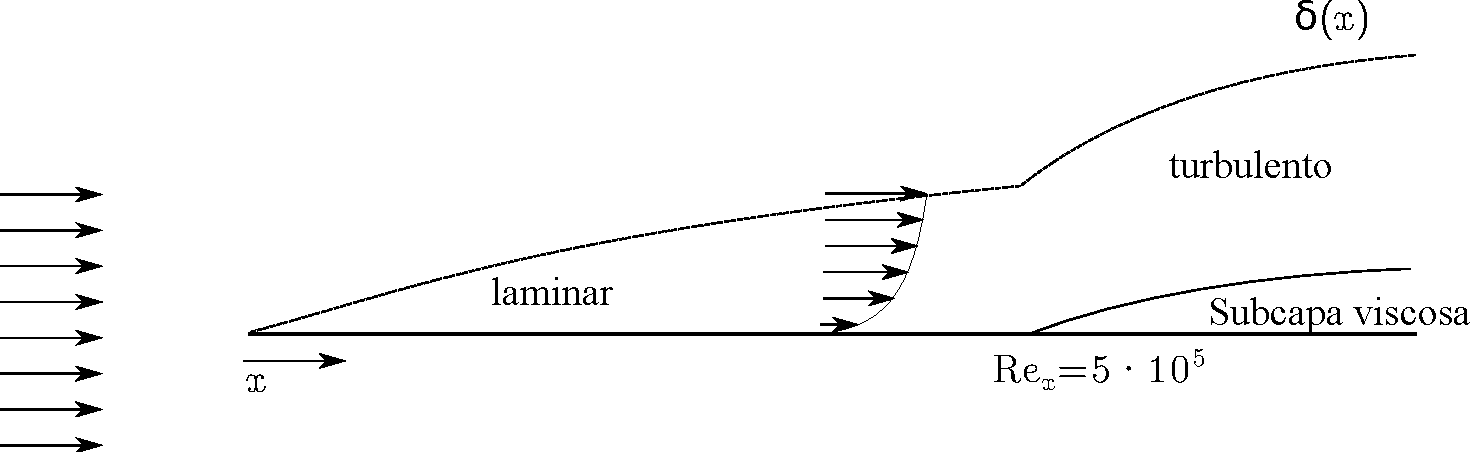
\includegraphics[width=0.8\textwidth]{clase05/capa_limite_Re.pdf}
\caption{Capa límite en función de $Re_x$.}
\label{fig:capa_limite_Re}
\end{figure}

Cuando la capa límite se torna turbulenta, aparece una pequeña zona laminar, pegada a la placa, que se conoce como subcapa viscosa.
Aparte de ser laminar, esta zona tiene importantes implicancias en el patrón del flujo dentro de la capa límite, ya que, si su espesor es mayor que la rugosidad de la placa, esta rugosidad no afecta al flujo y se puede considerar como una placa lisa. 
Como pueden imaginarse, esto tiene un importante efecto en el arrastre sobre la placa.

A continuación veremos algunas soluciones de capa límite, que dependen del número de Reynolds definido en la Ec. \eqref{eq:Re_capa}, tanto para flujo laminar, como para turbulento.

\section*{Ecuaciones en la capa límite}
En esta sección veremos como se reducen las ecuacines de conservación para el caso de flujo en una capa límite.
Para nuestro análisis, este flujo es incompresible, bidimiensional y estacionario, para lo cual continuidad y Navier-Stokes quedan como
%
\begin{align}\label{eq:NS_capa}
\frac{\partial u}{\partial x} + \frac{\partial v}{\partial y} &= 0 \nonumber\\
u\frac{\partial u}{\partial x} + v\frac{\partial u}{\partial y} &= -\frac{1}{\rho}\frac{\partial p}{\partial x} + \nu\left( \frac{\partial^2u}{\partial x^2} + \frac{\partial^2u}{\partial y^2}\right) \nonumber\\
u\frac{\partial v}{\partial x} + v\frac{\partial v}{\partial y} &= -\frac{1}{\rho}\frac{\partial p}{\partial y} + \nu\left( \frac{\partial^2v}{\partial x^2} + \frac{\partial^2v}{\partial y^2}\right).
\end{align}

Empecemos con aproximaciones propias de flujo en una capa límite.
En primer lugar, a pesar que es un flujo bidimensional, hay una clara dirección preferente ($x$ por sobre $y$).
Por esto, podemos esperar que $u>>v$.
Además, las variaciones en el eje perpendicular a la placa deben ser muchísimo más drásticas que en el eje paralelo a la placa:
%
\begin{equation}
\frac{\partial u}{\partial x} << \frac{\partial u}{\partial y}, \quad \frac{\partial v}{\partial x} << \frac{\partial v}{\partial y}, \quad \frac{\partial^2 u}{\partial x^2} << \frac{\partial^2 u}{\partial y^2}
\end{equation}

Por parte de la presión, nos ayuda mucho lo que ya sabemos de flujo no viscoso. 
Afuera de la capa límite tenemos prácticamente un flujo uniforme, igual al flujo potencial, donde la ecuación de Bernoulli es válida:
%
\begin{equation}
\frac{\partial p}{\partial x} = -\frac{\partial}{\partial x}\left(\rho \frac{U_\infty^2}{2}\right) = - \rho\frac{\partial U_\infty}{\partial x} = -\rho U_\infty\frac{dU_\infty}{dx} 
\end{equation}

Con estas aproximaciones, la Ec. \eqref{eq:NS_capa} queda
%
\begin{align}\label{eq:NS_capa_x}
\frac{\partial u}{\partial x} + \frac{\partial v}{\partial y} &= 0 \nonumber\\
u\frac{\partial u}{\partial x} + v\frac{\partial u}{\partial y} &\approx U_\infty \frac{dU_\infty}{dx} + \nu \frac{\partial^2u}{\partial y^2},
\end{align}
%
y condiciones de borde
%
\begin{align}
u &= v = 0 \text{ en } y=0\nonumber\\
u &= U_\infty \text{ en } y=\delta.
\end{align}

La Ec. \eqref{eq:NS_capa_x} solamente menciona el eje $x$.
En el eje $y$, al aplicar las mismas aproximaciones llegamos a una aseveración muy potente:
%
\begin{equation}\label{eq:NS_capa_y}
\frac{\partial p}{\partial y} = 0,
\end{equation}
%
lo que nos dice que la presión es constante dentro de la capa límite, a medida que nos alejamos de la placa.
Esto es algo que sin darse cuenta, ya han visto experimentalmente (o lo verán pronto).
Cuando midieron la presión en la superficie del cilindro en el laboratorio, se dieron cuenta que el flujo potencial es una muy buena aproximación.
El flujo potencial es no viscoso, sin embargo, la condición de no deslizamiento se debe haber estado enforzando \mbox{?`}Cómo flujo potencial es una buena aproximación?
La Ec. \eqref{eq:NS_capa_y} nos dice que la presión sobre la superficie del cilindro es igual al punto en el borde de la capa límite, normal al cilindro. 
El flujo fuera de la capa límite se representa muy bien por un flujo potencial, como ya hemos comentado, y es este flujo el que define la presión en la superficie del cilindro.

\section*{Solución de capa límite en flujo laminar --- Ecuación de Blasius}
La Ec. \eqref{eq:NS_capa_x} se puede resolver analíticamente para un flujo laminar y velocidad $U_\infty$ constante, la cual fue propuesta por Blasius (quien era estudiante de Prandtl) en 1908.
Blasius hizo el siguiente cambio de coordenadas
%
\begin{equation}\label{eq:f_blasius}
\frac{u}{U_\infty} = f'(\eta)
\end{equation}
%
donde 
%
\begin{equation}\label{eq:eta_blasius}
\eta = y\left(\frac{U_\infty}{\nu x}\right)^{1/2}.
\end{equation}
%
No sabemos mucho de la la función $f(\eta)$, pero viendo la Ec. \eqref{eq:eta_blasius}, nos podemos dar cuenta que lejos de la placa ($\eta\to\infty$ cuando $y\to\infty$), $u=U_\infty$, por lo tanto $f'(\infty) = 1$ según la Ec. \eqref{eq:f_blasius}.
Por otra parte, sobre la placa ($y=0$ y $\eta=0$) la velocidad $u=0$ por la condición de no deslizamiento, por lo que $f'(0)=0$.

Reemplacemos esta transformación en la Ec. \eqref{eq:NS_capa_x}.
Lo más fácil es encontrar $u$ y su derivada, estos son
%
\begin{align}\label{eq:u_blasius}
u &= U_\infty f'(\eta) \nonumber\\
\frac{\partial u}{\partial x} &= U_\infty f''(\eta)\frac{\partial \eta}{\partial x}\nonumber\\
\frac{\partial u}{\partial y} &= U_\infty f''(\eta)\frac{\partial \eta}{\partial y}\nonumber\\
\frac{\partial^2 u}{\partial y^2} &= U_\infty \left[f'''(\eta)\left(\frac{\partial \eta}{\partial y}\right)^2 + f''(\eta)\cancelto{0}{\frac{\partial^2\eta}{\partial y^2}}\right] = U_\infty f'''(\eta)\left(\frac{\partial \eta}{\partial y}\right)^2
\end{align}
%
donde
%
\begin{align}\label{eq:deta_dx}
\frac{\partial \eta}{\partial x} &= \frac{1}{2}y\left(\frac{U_\infty}{\nu x}\right)^{-1/2} \frac{-U_\infty}{\nu x^2} = -\frac{1}{2x} \eta\nonumber\\
\frac{\partial \eta}{\partial y} &= \left(\frac{U_\infty}{\nu x}\right)^{1/2}.
\end{align}

Para encontrar $v$, usaremos conceptos que aprendimos en flujo potencial.
Se acordarán que en un flujo incompresible, por continuidad, existe una función corriente $\psi$ tal que
%
\begin{equation}
u=\frac{\partial\psi}{\partial y}, \quad v=-\frac{\partial\psi}{\partial x}.
\end{equation}
%
Por lo tanto, a partir de la Ec. \eqref{eq:u_blasius} podemos encontrar una expresión para $\psi$
%
\begin{equation}\label{eq:psi_1}
\psi = \int u dy = U_\infty \left(\frac{\nu x}{U_\infty}\right)^{1/2}f(\eta).
\end{equation}

Calculemos $v$:
%
\begin{align}\label{eq:v_blasius}
v &= -\frac{\partial\psi}{\partial x} = -U_\infty\left[\frac{1}{2}\left(\frac{\nu x}{U_\infty}\right)^{-1/2}\frac{\nu}{U_\infty}f(\eta) + \left(\frac{\nu x}{U_\infty}\right)f'(\eta)\frac{\partial \eta}{\partial x}\right] \nonumber\\
& = -U_\infty\left[\frac{1}{2}\left(\frac{\nu}{U_\infty x}\right)^{1/2} f(\eta) - \left(\frac{\nu x}{U_\infty}\right)^{1/2}f'(\eta)\frac{\eta}{2x}\right] \nonumber\\  
& = -U_\infty\frac{1}{2}\left(\frac{\nu}{U_\infty x}\right)^{1/2} \left[f(\eta) - f'(\eta)\eta\right]
\end{align}
%
Al aplicar la condición de borde $v=0$ sobre la placa ($\eta=0$), llegamos a
%
\begin{equation}
0 = -U_\infty\frac{1}{2}\left(\frac{\nu}{U_\infty x}\right)^{1/2} f(0)
\end{equation}
%
lo que nos entrega la condición de contorno $f(0)=0$.

Reemplazando las Ecs. \eqref{eq:u_blasius}, \eqref{eq:deta_dx} y \eqref{eq:v_blasius} en la Ec. \eqref{eq:NS_capa_x} para $dU_\infty/dx = 0$, nos da:
%
\begin{equation}
-U_\infty f'U_\infty f''\frac{\eta}{2x} - \frac{U_\infty}{2}\left(\frac{\nu}{U_\infty x}\right)^{1/2}(f-f'\eta)U_\infty f''\left(\frac{U_\infty}{\nu x}\right)^{1/2} = \nu U_\infty f'''\left(\frac{U_\infty}{\nu x}\right).
\end{equation}
%
Noten que en esta última ecuación no escribimos el argumento de la función $f$ por comodidad.
Cancelando los términos correspondientes, llegamos a la ecuación de Blasius
%
\begin{equation}
f'''+\frac{ff''}{2}=0
\end{equation}

\section*{Espesor de capa límite de Blasius}

Recién llegamos a la ecuación de Blasius, que describe el perfil de velocidad dentro de la capa límite sobre una placa plana sin gradiente de presión:
 %
 \begin{align}\label{eq:blasius2}
f'''&+\frac{1}{2}ff''=0\nonumber\\
f'(\eta) &= \frac{u}{U_\infty} \nonumber\\
\eta &= y\left(\frac{U_\infty}{\nu x}\right)^{1/2}\nonumber\\
f(0) &= 0\nonumber\\
f'(0) &= 0\nonumber\\
f'(\infty) &= 1
 \end{align}

 La ecuacion de Blasius es una ecuación diferencial ordinaria que no tiene solución analítica, sin embargo, podemos resolverla numéricamente.
 Si se fijan en el código del repositorio Github,\footnote{\url{https://github.com/cdcooper84/mec220/blob/master/apuntes/clase05/blasius.ipynb}} verán  que resolvemos esta ecuación con un método de Euler, y que el borde de la capa límite (donde $u=0.99U_\infty$), se da para $\eta=5$.
En este punto $y=\delta$, y reemplazando en la Ec. \eqref{eq:blasius2} llegamos a
%
\begin{equation}\label{eq:delta_blasius}
\frac{\delta}{x} = \frac{5}{\sqrt{Re_x}}
\end{equation}

Comparando el espesor de capa límite de von Kármán (que asume un perfil parabólico) y la Ec. \eqref{eq:delta_blasius}, nos podemos dar cuenta que la solución dada por von Kármán, que asume un perfil parabólico, no está tan lejos de la solución real.
En el caso de von Kármán, llegamos a un factor $5.5$ y en Blasius de $5$, solamente un 10\% de diferencia.
Además, vemos en la Figura \ref{fig:capa_limite_blasius} que el perfil parabólico de von Kármán (línea punteada) es una buena aproximación del perfil de Blasius (línea sólida) dentro de la capa límite.
%
\begin{figure}
\centering
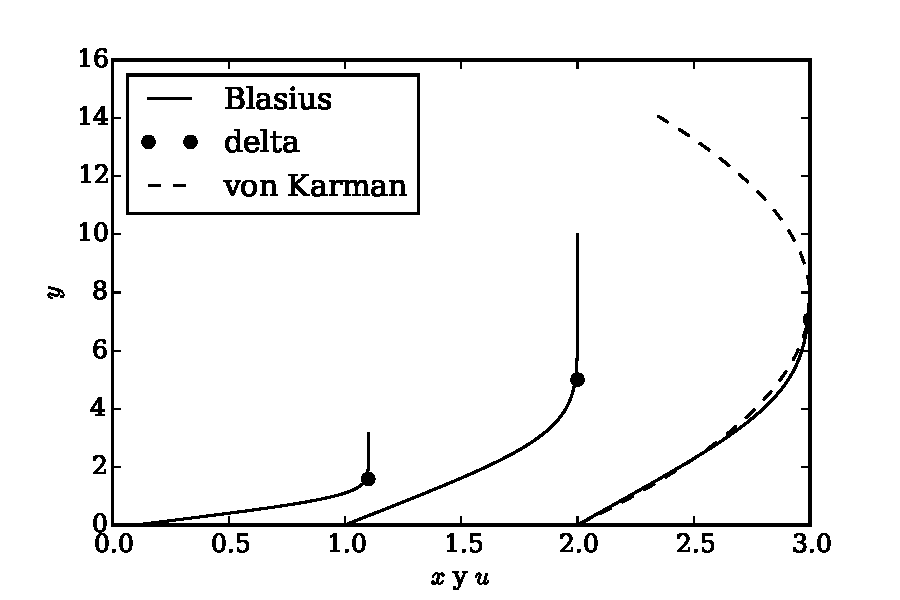
\includegraphics[width=0.7\textwidth]{clase05/capa_limite_blasius.pdf}
\caption{Perfil de velocidad dentro de la capa límite para $x=0.1$, $x=1$ y $x=2$. Línea sólida representa el perfil de Blasius, los puntos sólidos el fin de la capa límite, y la línea punteada el perfil parabólico de von Kármán.}
\label{fig:capa_limite_blasius}
\end{figure}

\paragraph*{Espesor de desplazamiento}

El espesor de desplazamiento de define como 
%
\begin{equation}
\delta^* = \int_0^\infty\left(1-\frac{u(y)}{U_\infty}\right)dy
\end{equation}
%
lo cual podemos reescribir en términos de $f(\eta)$, con $dy = d\eta\left(\frac{\nu x}{U_\infty}\right)^{1/2}$
%
\begin{align}
\delta^* &= \left(\frac{\nu x}{U_\infty}\right)^{1/2}\int_0^\infty(1-f'(\eta))d\eta\\
& = \left.\left(\frac{\nu x}{U_\infty}\right)^{1/2} (\eta-f(\eta))\right|_\infty
\end{align}

Usando el mismo código que antes, nos damos cuenta que al infinito el valor de $\eta-f'(\eta)$ tiende a 1.721, y podemos escribir
%
\begin{equation}
\frac{\delta^*}{x} = \frac{1.721}{\sqrt{Re_x}}
\end{equation}

\paragraph*{Esfuerzo cortante.}
Sabemos que la definición de $\tau_w$ es
%
\begin{equation}
\tau_w = \left.\mu\frac{du}{dy}\right|_0
\end{equation}
%
lo cual se puede escribir en términos de $f$ y $\eta$ como
%
\begin{align}
\tau_w &= \left. U_\infty\mu \frac{df'}{dy}\right|_0 = U_\infty\mu \left(\frac{U_\infty}{\nu x}\right)^{1/2}f''(0) \nonumber\\
&= U_\infty^{3/2}\left(\frac{\mu\rho}{x}\right)^{1/2}f''(0) = 0.332055 U_\infty^{3/2}\left(\frac{\mu\rho}{x}\right)^{1/2} 
\end{align}
%
Por otra parte, el coeficiente de arrastre es
%
\begin{equation}
c_f = \frac{\tau_w}{\frac{1}{2}U_\infty^2\rho} = \frac{2\cdot0.332055}{\sqrt{Re_x}} = \frac{0.664}{\sqrt{Re_x}}
\end{equation}

\paragraph*{Espesor de momentum.}
En la definición del espesor de momentum dijimos que
%
\begin{equation}
\tau_w = \rho U_\infty^2 \frac{d\theta}{dx}
\end{equation}
%
y usando la expresión que encontramos recién para $\tau_w$, quedamos con
%
\begin{align}
\theta &= \int_0^x 0.332 U_\infty^{3/2}\left(\frac{\mu\rho}{x}\right)^{1/2} \frac{1}{\rho U_\infty^2} dx \nonumber\\
&= \int_0^x 0.332 \left(\frac{\mu}{xU_\infty\rho}\right)^{1/2} dx = 2\cdot0.332 x^{1/2}\left(\frac{\mu}{U_\infty\rho}\right)^{1/2}
\end{align}
%
y dividiendo por $x$, queda
%
\begin{equation}
\frac{\theta}{x} = \frac{0.664}{\sqrt{Re_x}}
\end{equation}

 
\end{document}
